\documentclass[12pt]{article}
\usepackage{amsmath}
\usepackage{graphicx}
\usepackage{xcolor}
\usepackage[a4paper, total={7in, 8in}]{geometry}
\usepackage{amsmath}
\usepackage{amsfonts}
\graphicspath{ {./images/} }

\newtheorem{theorem}{Theorem}

\DeclareMathOperator{\Tr}{Tr}

\begin{document}
    \begin{center}
        Homework 1: Dmytrenko Dmytrenko
    \end{center}

    \begin{theorem}
        Denote by $\delta = \det A$, $\tau = \Tr A$
        and $\dot{x} = Ax$ then:
        \begin{itemize}
            \item saddle if $\delta < 0$
            \item node (stable for $\tau<0$ and
            unstable for $\tau>0$) if 
            $\begin{cases}
                \delta > 0\\
                \tau^2-4\delta\geq 0
            \end{cases}$
            \item focus (stable for $\tau<0$ and
            unstable for $\tau>0$) if 
            $\begin{cases}
                \delta > 0\\
                \tau^2-4\delta < 0\\
                \tau\neq 0
            \end{cases}$
            \item center if  
            $\begin{cases}
                \delta > 0\\
                \tau = 0
            \end{cases}$
        \end{itemize}
    \end{theorem}

    % ----------------------Ex1-----------------------
    \textbf{Exercise 1}
    $$
        A =
        \begin{pmatrix}
            3 & 1\\
            1 & 3
        \end{pmatrix}
    $$

    First of all, we should solve the corresponding
    characteristic equation
    $$
        \det (A - \lambda I) = 
        \begin{vmatrix}
            3-\lambda & 1\\
            1 & 3-\lambda
        \end{vmatrix}
        = (3-\lambda)^2-1
        =(\lambda-4)(\lambda-2)
    $$

    So, $\lambda_1 = 2$ and $\lambda_1 = 4$. 
    Corresponding eigenvectors are 
    $v_1 = (-1,1)^T$ and $v_2 = (1,1)^T$. Then
    $$
        B = PAP^{-1} =
        \begin{pmatrix}
            2 & 0\\
            0 & 4
        \end{pmatrix}
    $$

    $$
        x(t) = 
        \begin{pmatrix}
            e^{2t} & 0\\
            0 & e^{4t}
        \end{pmatrix}
        x_0
    $$

    After that, observe
    $$
        \delta = 8,\quad\tau = 6
    $$
    $$
        \delta > 0,\quad\tau > 0,\quad
        \tau^2-4\delta>0
    $$

    Thus, using theorem, we have \textit{unstable node} 
    and phase portrait consists of trajectories
    $x_1 = x_2$, $x_1 = -x_2$ and set of parabols.

    \begin{center}
        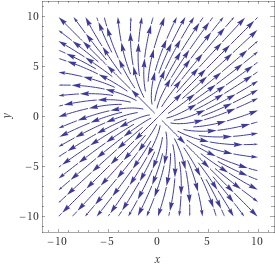
\includegraphics[scale=0.75]{plot1.png}
    \end{center}

    Finally,
    $$
        E^u = span
        \left\{ 
            \begin{pmatrix}
                -1\\
                1
            \end{pmatrix},
            \begin{pmatrix}
                1\\
                1
            \end{pmatrix}
        \right\},
        \quad
        E^s=\emptyset
    $$

    % ----------------------Ex2-----------------------

    \textbf{Exercise 2}
    $$
        A =
        \begin{pmatrix}
            2 & 4\\
            -1 & 2
        \end{pmatrix}
    $$

    First of all, we should solve the corresponding
    characteristic equation

    $$
        \det (A - \lambda I) = 
        \begin{vmatrix}
            2-\lambda & 4\\
            -1 & 2-\lambda
        \end{vmatrix}
        = (2-\lambda)^2+4
        =\lambda^2 -4\lambda +8
    $$

    So, $\lambda_1 = 2-2i$ and $\lambda_1 = 2+2i$.
    Then
    
    $$
        B = PAP^{-1} =
        \begin{pmatrix}
            2 & -2\\
            2 & 2
        \end{pmatrix}
    $$
    
    $$
        x(t) = e^{2t}
        \begin{pmatrix}
            \cos 2t & -\sin 2t\\
            \sin 2t & \cos 2t
        \end{pmatrix}
        x_0
    $$

    After that, observe
    $$
        \delta = 8,\quad\tau = 4
    $$
    $$
        \delta>0,\quad\tau > 0,\quad
        \tau^2-4\delta>0
    $$

    Thus, using theorem, we have \textit{unstable node}.
    Computing velocity vector at arbitrary point (1,0)
    $$  
        \left.
        \begin{pmatrix}
            \dot{x_1}\\
            \dot{x_2}
        \end{pmatrix}
        \right\vert_{(1,0)} =
        \begin{pmatrix}
            2\\
            -1
        \end{pmatrix}
    $$
    our phase portrait looks like
    
    \begin{center}
        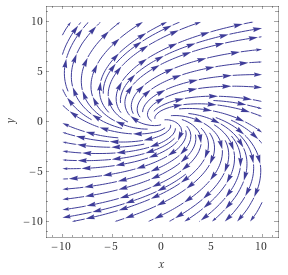
\includegraphics{plot2.png}
    \end{center}

    Finally, $E^u=x_1 x_2$ plane and $E^s=\emptyset$

    % ----------------------Ex3-----------------------

    \textbf{Exercise 3}
    $$
        A =
        \begin{pmatrix}
            1 & 0 & 0\\
            1 & 2 & 0\\
            1 & 0 & -1
        \end{pmatrix}
    $$

    First of all, we should solve the corresponding
    characteristic equation

    $$
        \det (A - \lambda I) = 
        \begin{pmatrix}
            1-\lambda & 0 & 0\\
            1 & 2-\lambda & 0\\
            1 & 0 & -1-\lambda
        \end{pmatrix} =
        -\lambda^3+2\lambda^2+\lambda-2
    $$

    So, $\lambda_1 = 2$, $\lambda_2 = -1$
    and $\lambda_3 = 1$. Corresponding eigenvectors are 
    $v_1 = (0,1,0)^T$, $v_2 = (0,0,1)^T$, $v_3 = (2,-2,1)^T$ and
     . Then

    $$
        P =
        \begin{pmatrix}
            0 & 0 &  2\\
            1 & 0 & -2\\
            0 & 1 &  1
        \end{pmatrix}
    $$

    $$
        P^{-1} =
        \begin{pmatrix}
            1 & 1 & 0\\
            -\frac{1}{2} & 0 & 1\\
            \frac{1}{2} & 0 & 0
        \end{pmatrix}
    $$
    
    $$
        B = PAP^{-1} =
        \begin{pmatrix}
            2 & 0 & 0\\
            0 & -1 & 0\\
            0 & 0 & 1
        \end{pmatrix}
    $$

    $$
        x(t) = 
        \begin{pmatrix}
            e^{2t} & 0 & 0\\
            0 & e^{-t} & 0\\
            0 & 0 & e^{t}
        \end{pmatrix}
        x_0
    $$

    After that, observe
    $$
        \delta = -2,\quad\tau = 0
    $$
    $$
        \delta < 0,\quad\tau = 0,\quad
        \tau^2-4\delta>0
    $$

    Thus, using theorem, we have \textit{saddle}.

    \begin{center}
        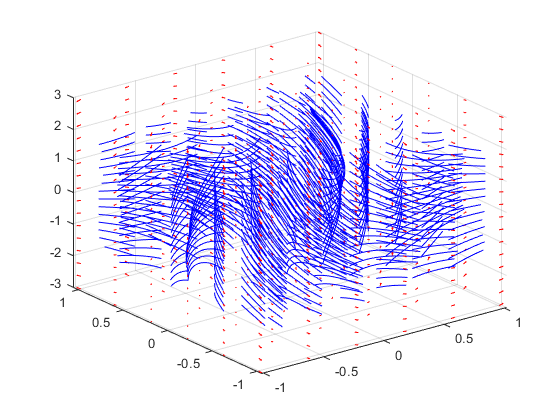
\includegraphics[scale=0.8]{plot3.png}
    \end{center}

    Finally,
    $$
        E^u = span
        \left\{ 
            \begin{pmatrix}
                0\\
                1\\
                0
            \end{pmatrix},
            \begin{pmatrix}
                0\\
                0\\
                1
            \end{pmatrix},
            \begin{pmatrix}
                2\\
                -2\\
                1
            \end{pmatrix}
        \right\},
        \quad
        E^s=\emptyset
    $$

    % ----------------------Ex4-----------------------

    \textbf{Exercise 4}
    $$
        A =
        \begin{pmatrix}
            0 & -2 & 0\\
            1 & 2 & 0\\
            0 & 0 & -2
        \end{pmatrix}
    $$

    First of all, we should solve the corresponding
    characteristic equation

    $$
        \det (A - \lambda I) = 
        \begin{pmatrix}
            -\lambda & -2 & 0\\
            1 & 2-\lambda & 0\\
            1 & 0 & -2-\lambda
        \end{pmatrix} =
        -\lambda^3+2\lambda^2+\lambda-2
    $$

    So, $\lambda_1 = -2$, $\lambda_2 = 1-i$
    and $\lambda_3 = 1+i$. Corresponding eigenvectors are 
    $v_1 = (0,0,1)^T$, 
    $
        v_{2,3} = 
        \begin{pmatrix}
            -1\\
            1\\
            0        
        \end{pmatrix} + i
        \begin{pmatrix}
            1\\
            0\\
            0
        \end{pmatrix}
    $. Then

    $$
        P =
        \begin{pmatrix}
            0 & 1 &  -1\\
            0 & 0  &  1\\
            1 & 0  &  0
        \end{pmatrix}
    $$

    $$
        P^{-1} =
        \begin{pmatrix}
            0 & 0 & 1\\
            -1 & -1 & 0\\
            0 & 1 & 0
        \end{pmatrix}
    $$
    
    $$
        B = PAP^{-1} =
        P\cdot
        \begin{pmatrix}
            0 & e^t\cos t & -e^t\sin t\\
            0 & e^t\sin t & e^t\cos t\\
            e^t & 0 & 0
        \end{pmatrix}
        \cdot P^{-1}
    $$

    $$
        x(t) = 
        B\cdot
        x_0
    $$

    After that, observe
    $$
        \delta = -4,\quad\tau = 0
    $$
    $$
        \delta < 0,\quad\tau = 0,\quad
        \tau^2-4\delta>0
    $$
    
    Thus, using theorem, we have \textit{saddle}.

    \begin{center}
        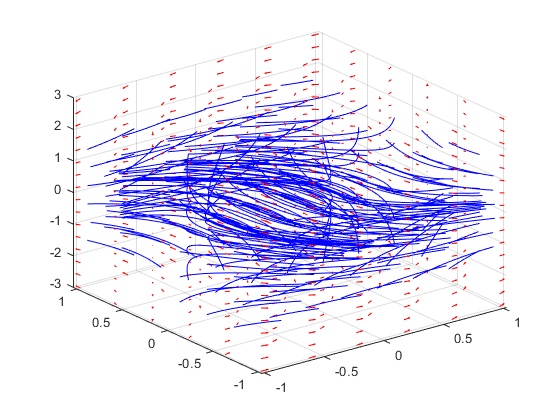
\includegraphics[scale=0.69]{plot4.png}
    \end{center}

    Finally,
    $Re\lambda_{1,2,3}<0$.

    $$
        E^u = span
        \left\{ 
            \begin{pmatrix}
                0\\
                0\\
                1
            \end{pmatrix},
            \begin{pmatrix}
                1\\
                0\\
                0
            \end{pmatrix},
            \begin{pmatrix}
                -1\\
                1\\
                0
            \end{pmatrix}
        \right\},
        \quad
        E^s=\emptyset
    $$

    % ----------------------Ex5-----------------------

    \textbf{Exercise 5}
    $$
        A =
        \begin{pmatrix}
            1 & 0 & 0\\
            -1 & 2 & 0\\
            1 & 1 & 2
        \end{pmatrix}
    $$

    First of all, we should solve the corresponding
    characteristic equation

    $$
        \det (A - \lambda I) = 
        \begin{pmatrix}
            1-\lambda & 0 & 0\\
            -1 & 2-\lambda & 0\\
            1 & 1 & 2-\lambda
        \end{pmatrix} =
        -\lambda^3+5\lambda^2-8\lambda+4
    $$

    So, $\lambda_1 = 1$ and $\lambda_{2,3} = 2$. 
    Corresponding eigenvectors are 
    $   v_1 = 
        \begin{pmatrix}
            -1\\
            -1\\
            2
        \end{pmatrix}
    $, 
    $
        v_{2,3} = 
        \begin{pmatrix}
            0\\
            0\\
            1        
        \end{pmatrix}
    $. 
    
    Because of $\lambda_{2,3}=2$ has multiplicity
    2, then we need to find extra generalized
    eigenvector of A when $\lambda=2$ and $k=2$
    $$
        (A-\lambda I)^k\cdot v=
        \begin{pmatrix}
            -1 & 0 & 0\\
            -1 & 0 & 0\\
            1 & 1 & 0
        \end{pmatrix}^2\cdot v=
        \begin{pmatrix}
            -1 & 0 & 0\\
            -1 & 0 & 0\\
            1 & 1 & 0
        \end{pmatrix}\cdot
        \begin{pmatrix}
            -1 & 0 & 0\\
            -1 & 0 & 0\\
            1 & 1 & 0
        \end{pmatrix}\cdot
        \begin{pmatrix}
            v_1\\
            v_2\\
            v_3 
        \end{pmatrix}=
    $$

    $$
        \begin{pmatrix}
            1 & 0 & 0\\
            1 & 0 & 0\\
            0 & 0 & 0
        \end{pmatrix}\cdot
        \begin{pmatrix}
            v_1\\
            v_2\\
            v_3 
        \end{pmatrix}\implies
        \begin{pmatrix}
            v_1\\
            v_2\\
            v_3 
        \end{pmatrix}=
        \begin{pmatrix}
            0\\
            1\\
            1 
        \end{pmatrix}
    $$

    So, now we obtain:
    $$
        P =
        \begin{pmatrix}
            -1 & 0 & 0\\
            -1 & 0 & 1\\
             2 & 1 & 1
        \end{pmatrix}
    $$

    $$
        P^{-1} =
        \begin{pmatrix}
            -1 &  0 & 0\\
             3 & -1 & 1\\
            -1 &  1 & 0
        \end{pmatrix}
    $$
    
    Then

    $$
        S =
        \begin{pmatrix}
            1  & 0 &  0\\
            0 & 2 &  0\\
            0  & 0 &  2
        \end{pmatrix}
    $$

    $$
        N = A - S =
        \begin{pmatrix}
            1 & 0 & 0\\
            -1 & 2 & 0\\
            1 & 1 & 2
        \end{pmatrix} -
        \begin{pmatrix}
            1  & 0 &  0\\
            0 & 2 &  0\\
            0  & 0 &  2
        \end{pmatrix} =
        \begin{pmatrix}
            0  & 0 &  0\\
            -1 & 0 &  0\\
            1  & 1 &  0
        \end{pmatrix}
    $$
    
    $$
        N^2 = N\cdot N = 
        \begin{pmatrix}
            0  & 0 &  0\\
            -1 & 0 &  0\\
            1  & 1 &  0
        \end{pmatrix}\cdot
        \begin{pmatrix}
            0  & 0 &  0\\
            -1 & 0 &  0\\
            1  & 1 &  0
        \end{pmatrix} =
        \begin{pmatrix}
            0  & 0 &  0\\
            0 & 0 &  0\\
            -1  & 0 &  0
        \end{pmatrix}
    $$

    $$
        N^3 = N^2 \cdot N = 
        \begin{pmatrix}
            0  & 0 &  0\\
            0 & 0 &  0\\
            -1  & 0 &  0
        \end{pmatrix}\cdot
        \begin{pmatrix}
            0  & 0 &  0\\
            -1 & 0 &  0\\
            1  & 1 &  0
        \end{pmatrix} =
        \begin{pmatrix}
            0  & 0 &  0\\
            0  & 0 &  0\\
            0  & 0 &  0
        \end{pmatrix}
    $$

    So, N is nilpotent of order k=3.

    Thus,
    $$
        x(t)=P\cdot diag\left[e^{\lambda_1 t} e^{\lambda_2 t} e^{\lambda_3 t}\right]
        \cdot P^{-1}\cdot\left[I + Nt +\dfrac{N^2 t^2}{2}\right]x_0
    $$

    $$
        x(t)=
        \begin{pmatrix}
            -1 & 0 & 0\\
            -1 & 0 & 1\\
             2 & 1 & 1
        \end{pmatrix}\cdot
        \begin{pmatrix}
            e^{t} & 0 & 0\\
            -1 & e^{2t} & 0\\
            0 & 0 & e^{2t}
        \end{pmatrix}\cdot
        \begin{pmatrix}
            -1 &  0 & 0\\
             3 & -1 & 1\\
            -1 &  1 & 0
        \end{pmatrix}\cdot
        \begin{pmatrix}
            1 &  0 & 0\\
            -t & 1 & 0\\
            t-\frac{t^2}{2} &  t & 1
        \end{pmatrix}
        x_0
    $$

    After that, observe
    $$
        \delta = 4,\quad\tau = 5
    $$
    $$
        \delta>0,\quad\tau > 0,\quad
        \tau^2-4\delta>0
    $$

    Thus, using theorem, we have \textit{unstable node}.
    \begin{center}
        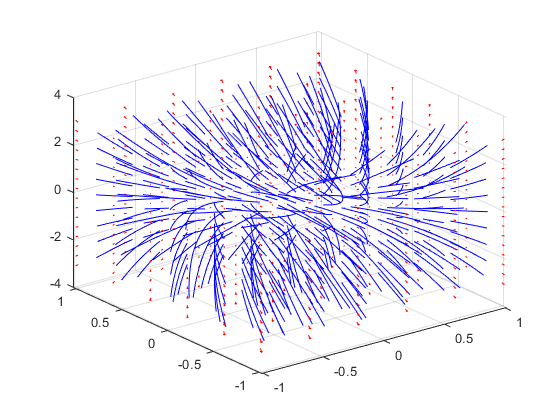
\includegraphics[scale=0.7]{plot5.png}
    \end{center}

    Finally,
    $\lambda_{1,2,3}>0$.

    $$
        E^u = \text{our space}\:x_1,x_2,x_3;
        \quad
        E^s=\emptyset
    $$
    
\end{document}